\documentclass{standalone}
\usepackage{tikz}


\begin{document}
        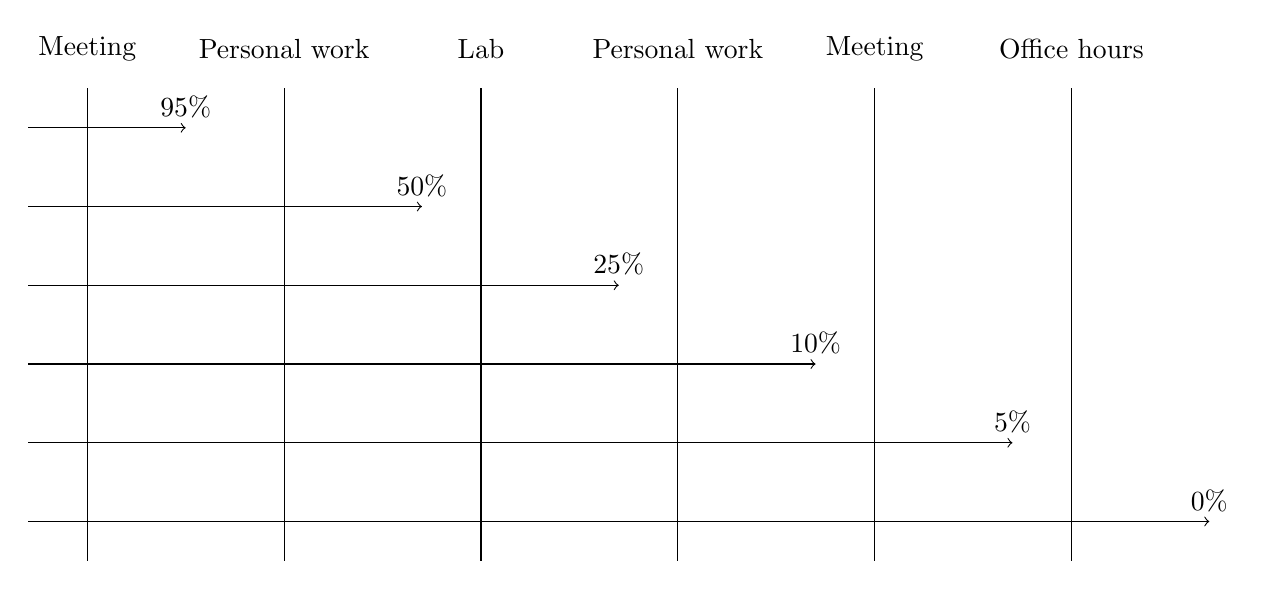
\begin{tikzpicture}
            \foreach \i/\label in {2.5/Meeting,
                                   5/Personal work,
                                   7.5/Lab,
                                   10/Personal work,
                                   12.5/Meeting,
                                   15/Office hours}
                {
                    \draw (\i, -5) -- (\i, 1);
                    \node at (\i, 1.5) {\label};
                }

            \draw [->] (1.75, .5) -- node [above, at end] {95\%} (3.75, .5);
            \draw [->] (1.75, -.5) -- node [above, at end] {50\%} (6.75, -.5);
            \draw [->] (1.75, -1.5) -- node [above, at end] {25\%} (9.25, -1.5);
            \draw [->] (1.75, -2.5) -- node [above, at end] {10\%} (11.75, -2.5);
            \draw [->] (1.75, -3.5) -- node [above, at end] {5\%} (14.25, -3.5);
            \draw [->] (1.75, -4.5) -- node [above, at end] {0\%} (16.75, -4.5);
    \end{tikzpicture}
\end{document}
